\documentclass[12pt]{beamer}

    \usepackage[utf8]{inputenc}
    \usepackage{graphics}
    \usepackage{listings}
    
    \usepackage{array,booktabs}
    
    \usetheme{Madrid}
    \usecolortheme{beaver}
    
    % custom commands
    \newcommand{\nologo}{\setbeamertemplate{logo}{}} % set logo to empty
    
    \title{Airflow}
    \author{Arun}
    \date{\today}
    
    
    \logo{
\includegraphics[height=1.0cm]{images/logo.png}}
    
    \begin{document}
        \frame{\titlepage}
        \begin{frame}
            \begin{center}
                \huge{Airflow}
            \end{center}
        \end{frame}
    
        \begin{frame}
            \begin{center}
                \frametitle{What is Airflow?}
                \begin{itemize}
                    \pause
                    \item It's a workflow manager
                    \pause
                    \item We can also call it a fancy Scheduler
                    \pause
                    \item It can be a easy backend job Scheduler in a distributed system
                    \item Ref, \href{https://medium.com/@rako/apache-airflow-as-an-external-scheduler-for-distributed-systems-53b7354d3e48}{this blog}
                \end{itemize}
            \end{center}
        \end{frame}
    
        \begin{frame}
            \begin{center}
                \frametitle{Other tools}
                \begin{itemize}
                    \pause
                    \item Oozie - XML code
                    \pause
                    \item Pinball (pinterest) - no community interest
                    \pause
                    \item Luigi (Spotify) - Uses HDFS, no alerts or monitoring
                    \pause
                    \item Azkaban (LinkedIn) - Uses custom config file for workflow setups
                \end{itemize}
            \end{center}
        \end{frame}
    
        \begin{frame}
            \frametitle{Airflow}
            \begin{itemize}
                \pause
                \item Python code base + for workflow definitions
                \pause
                \item Trigger rules
                \pause
                \item Xcoms
                \pause
                \item Cool UI \& CLI
                \pause
                \item Queues \& Pools
                \pause
                \item Zombie cleanup
                \pause
                \item Large community
            \end{itemize}
        \end{frame}
        
        \begin{frame}
            \begin{center}
                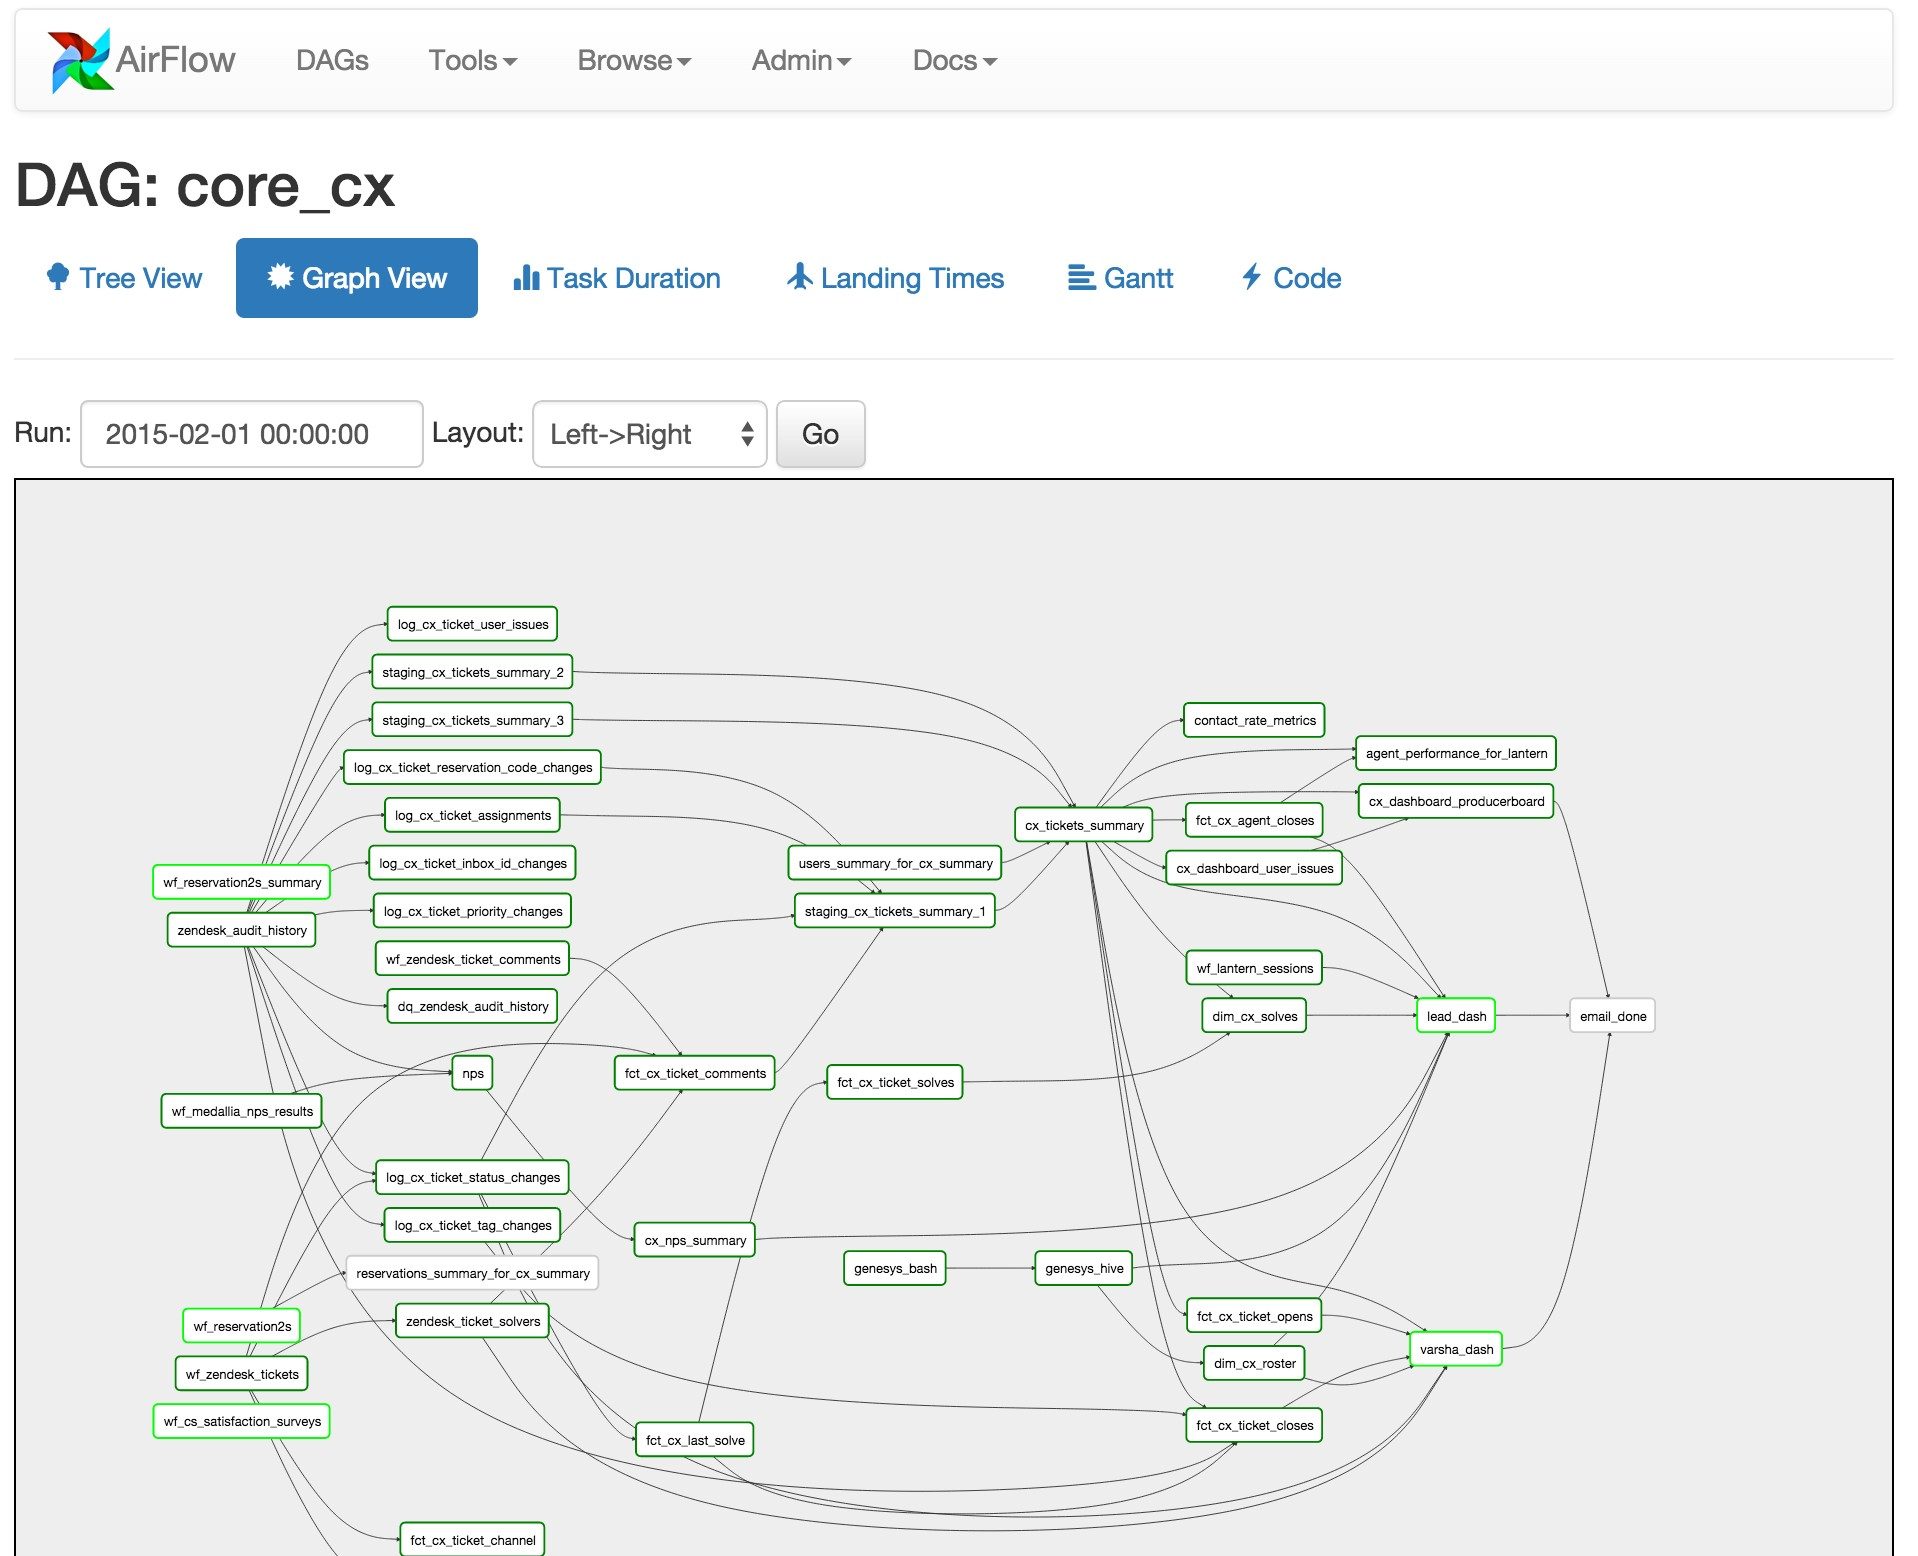
\includegraphics[width=1\textwidth]{images/workflow.png}
            \end{center}
        \end{frame}

        \begin{frame}
            \frametitle{Airflow - Executors}
            \begin{itemize}
                \item Sequential
                \item Local (parallel)
                \item Celery
                \item Mesos
                \item Kubernetes (still in alpha)
            \end{itemize}
        \end{frame}

        \begin{frame}
            \frametitle{Our cluster}
            \begin{itemize}
                \item Single node (8 core, 20 GB node)
                \item Local Executor (with 24 parallel schedulable tasks)
                \item 3000+ tasks triggred a day
                \item Code auto deployed from master to prod
            \end{itemize}
        \end{frame}

        \begin{frame}
            \frametitle{Tasks}
            \begin{itemize}
                \item BQ job
                \item Run spark jobs daily for ML
                \item All batched jobs in Google Dataflow
                \item Scheduling backend jobs
                \item All errors to SLACK
                \item Critical DAG failures will invoke Victorops issue
            \end{itemize}
        \end{frame}
    
    \end{document}
    